\documentclass[11pt]{article}

\usepackage[margin=0.7in]{geometry}

\usepackage{amsmath,booktabs,longtable,float,hyperref,siunitx}

\usepackage{xcolor}

\usepackage{pgfplots}

\pgfplotsset{compat=1.18}

\hypersetup{colorlinks=true,linkcolor=blue,urlcolor=blue}

\title{NF=10 / NF=1 Noise Simulation Combined Report}

\author{Codex analysis}

\date{2026-05-15 HKT}

\begin{document}

\maketitle

\section*{Executive Summary}

Both raw result sets are captured and archived: NF=10 / noisescale=10 sampling-noise stress mode and NF=1 / noisescale=1 full-noise mode. Each data set contains 20 completed points across four $t_d$ settings and five process corners. All Spectre points completed with 0 errors. The analysis below is corner-by-corner; averages are not used as the primary conclusion.

\section*{Noise Calculation}

Assume $V_{FS}=V_{ref}=1$ Vpp and 12 bits:
\begin{align*}
LSB &= V_{FS}/2^{12}=244.141\,\mu V \\
V_{q,rms} &= LSB/\sqrt{12}=70.477\,\mu V \\
P_q &= 4.967054\times10^{-9}\,V^2 \\
P_{sig} &= (V_{FS}/(2\sqrt{2}))^2=0.125000\,V^2 \\
P_{total} &= P_{sig}/10^{SNR/10} \\
P_{excess} &= \max(P_{total}-P_q,0)
\end{align*}
If $V_{FS}=2V_{ref}$ is used, RMS values scale by 2 and powers by 4; $t_d$ trends are unchanged.

\begin{table}[H]
\centering
\caption{Best $t_d$ by corner using SNR as the selection criterion.}
\begin{tabular}{lrrrrrr}
\toprule
Corner & NF10 $t_d$ & NF10 SNR & NF10 ENOB & NF1 $t_d$ & NF1 SNR & NF1 ENOB \\
\midrule
Nominal & 27n & 64.24 & 10.33 & 25n & 68.44 & 11.10 \\
C0 & 26n & 64.40 & 10.42 & 25n & 69.55 & 11.20 \\
C1 & 27n & 61.54 & 9.95 & 25n & 67.80 & 10.92 \\
fs & 26n & 64.86 & 10.46 & 25n & 69.12 & 11.16 \\
sf & 27n & 61.83 & 9.92 & 27n & 67.93 & 11.03 \\
\bottomrule
\end{tabular}
\end{table}

\section*{Figures}

\begin{figure}[H]
\centering
\begin{minipage}{0.49\linewidth}
\begin{tikzpicture}
\begin{axis}[
width=\linewidth, height=0.32\textheight,
xlabel={$\Delta t_d$ (ns)},
ylabel={SNR (dB)},
xmin=0, xmax=3.1,
grid=both,
legend style={font=\scriptsize, cells={anchor=west}},
legend pos=south east,
tick label style={font=\scriptsize},
label style={font=\small},
title style={font=\small},
title={NF=10 / noisescale=10}, ymin=50
]
\addplot+[mark=*] coordinates {(0.05,54.898) (1.00,59.542) (2.00,61.787) (3.00,64.244)};
\addlegendentry{Nominal}
\addplot+[mark=*] coordinates {(0.05,56.977) (1.00,62.915) (2.00,64.404) (3.00,63.801)};
\addlegendentry{C0}
\addplot+[mark=*] coordinates {(0.05,53.004) (1.00,57.216) (2.00,60.480) (3.00,61.544)};
\addlegendentry{C1}
\addplot+[mark=*] coordinates {(0.05,56.247) (1.00,61.772) (2.00,64.855) (3.00,63.720)};
\addlegendentry{fs}
\addplot+[mark=*] coordinates {(0.05,53.727) (1.00,58.080) (2.00,60.378) (3.00,61.830)};
\addlegendentry{sf}
\end{axis}
\end{tikzpicture}
\end{minipage}\hfill
\begin{minipage}{0.49\linewidth}
\begin{tikzpicture}
\begin{axis}[
width=\linewidth, height=0.32\textheight,
xlabel={$\Delta t_d$ (ns)},
ylabel={SNR (dB)},
xmin=0, xmax=3.1,
grid=both,
legend style={font=\scriptsize, cells={anchor=west}},
legend pos=south east,
tick label style={font=\scriptsize},
label style={font=\small},
title style={font=\small},
title={NF=1 / noisescale=1}, ymin=50
]
\addplot+[mark=*] coordinates {(0.05,67.952) (1.00,68.437) (2.00,67.390) (3.00,67.346)};
\addlegendentry{Nominal}
\addplot+[mark=*] coordinates {(0.05,68.508) (1.00,69.545) (2.00,68.385) (3.00,64.938)};
\addlegendentry{C0}
\addplot+[mark=*] coordinates {(0.05,67.518) (1.00,67.799) (2.00,67.439) (3.00,67.637)};
\addlegendentry{C1}
\addplot+[mark=*] coordinates {(0.05,68.188) (1.00,69.121) (2.00,68.461) (3.00,64.437)};
\addlegendentry{fs}
\addplot+[mark=*] coordinates {(0.05,67.931) (1.00,67.246) (2.00,67.084) (3.00,67.934)};
\addlegendentry{sf}
\end{axis}
\end{tikzpicture}
\end{minipage}
\caption{SNR versus $\Delta t_d$ by corner.}
\end{figure}

\begin{figure}[H]
\centering
\begin{minipage}{0.49\linewidth}
\begin{tikzpicture}
\begin{axis}[
width=\linewidth, height=0.32\textheight,
xlabel={$\Delta t_d$ (ns)},
ylabel={ENOB (bit)},
xmin=0, xmax=3.1,
grid=both,
legend style={font=\scriptsize, cells={anchor=west}},
legend pos=south east,
tick label style={font=\scriptsize},
label style={font=\small},
title style={font=\small},
title={NF=10 / noisescale=10}, ymin=8
]
\addplot+[mark=*] coordinates {(0.05,8.760) (1.00,9.531) (2.00,9.948) (3.00,10.333)};
\addlegendentry{Nominal}
\addplot+[mark=*] coordinates {(0.05,9.109) (1.00,10.141) (2.00,10.420) (3.00,10.332)};
\addlegendentry{C0}
\addplot+[mark=*] coordinates {(0.05,8.543) (1.00,9.234) (2.00,9.799) (3.00,9.948)};
\addlegendentry{C1}
\addplot+[mark=*] coordinates {(0.05,8.991) (1.00,9.890) (2.00,10.462) (3.00,10.270)};
\addlegendentry{fs}
\addplot+[mark=*] coordinates {(0.05,8.561) (1.00,9.311) (2.00,9.677) (3.00,9.916)};
\addlegendentry{sf}
\end{axis}
\end{tikzpicture}
\end{minipage}\hfill
\begin{minipage}{0.49\linewidth}
\begin{tikzpicture}
\begin{axis}[
width=\linewidth, height=0.32\textheight,
xlabel={$\Delta t_d$ (ns)},
ylabel={ENOB (bit)},
xmin=0, xmax=3.1,
grid=both,
legend style={font=\scriptsize, cells={anchor=west}},
legend pos=south east,
tick label style={font=\scriptsize},
label style={font=\small},
title style={font=\small},
title={NF=1 / noisescale=1}, ymin=8
]
\addplot+[mark=*] coordinates {(0.05,11.013) (1.00,11.103) (2.00,10.963) (3.00,10.943)};
\addlegendentry{Nominal}
\addplot+[mark=*] coordinates {(0.05,11.089) (1.00,11.204) (2.00,11.080) (3.00,10.484)};
\addlegendentry{C0}
\addplot+[mark=*] coordinates {(0.05,10.964) (1.00,10.921) (2.00,10.928) (3.00,10.890)};
\addlegendentry{C1}
\addplot+[mark=*] coordinates {(0.05,11.059) (1.00,11.162) (2.00,11.098) (3.00,10.401)};
\addlegendentry{fs}
\addplot+[mark=*] coordinates {(0.05,10.898) (1.00,10.871) (2.00,10.878) (3.00,11.026)};
\addlegendentry{sf}
\end{axis}
\end{tikzpicture}
\end{minipage}
\caption{ENOB versus $\Delta t_d$ by corner.}
\end{figure}

\begin{figure}[H]
\centering
\begin{minipage}{0.49\linewidth}
\begin{tikzpicture}
\begin{axis}[
width=\linewidth, height=0.32\textheight,
xlabel={$\Delta t_d$ (ns)},
ylabel={SFDR (dB)},
xmin=0, xmax=3.1,
grid=both,
legend style={font=\scriptsize, cells={anchor=west}},
legend pos=south east,
tick label style={font=\scriptsize},
label style={font=\small},
title style={font=\small},
title={NF=10 / noisescale=10}, ymin=60
]
\addplot+[mark=*] coordinates {(0.05,66.318) (1.00,69.765) (2.00,74.033) (3.00,75.278)};
\addlegendentry{Nominal}
\addplot+[mark=*] coordinates {(0.05,67.896) (1.00,73.921) (2.00,75.229) (3.00,74.814)};
\addlegendentry{C0}
\addplot+[mark=*] coordinates {(0.05,65.535) (1.00,67.936) (2.00,71.930) (3.00,72.968)};
\addlegendentry{C1}
\addplot+[mark=*] coordinates {(0.05,67.776) (1.00,72.561) (2.00,77.562) (3.00,74.767)};
\addlegendentry{fs}
\addplot+[mark=*] coordinates {(0.05,64.167) (1.00,69.511) (2.00,70.525) (3.00,73.576)};
\addlegendentry{sf}
\end{axis}
\end{tikzpicture}
\end{minipage}\hfill
\begin{minipage}{0.49\linewidth}
\begin{tikzpicture}
\begin{axis}[
width=\linewidth, height=0.32\textheight,
xlabel={$\Delta t_d$ (ns)},
ylabel={SFDR (dB)},
xmin=0, xmax=3.1,
grid=both,
legend style={font=\scriptsize, cells={anchor=west}},
legend pos=south east,
tick label style={font=\scriptsize},
label style={font=\small},
title style={font=\small},
title={NF=1 / noisescale=1}, ymin=60
]
\addplot+[mark=*] coordinates {(0.05,81.432) (1.00,76.687) (2.00,77.140) (3.00,78.346)};
\addlegendentry{Nominal}
\addplot+[mark=*] coordinates {(0.05,79.105) (1.00,78.695) (2.00,79.438) (3.00,76.730)};
\addlegendentry{C0}
\addplot+[mark=*] coordinates {(0.05,78.431) (1.00,79.667) (2.00,78.799) (3.00,79.841)};
\addlegendentry{C1}
\addplot+[mark=*] coordinates {(0.05,79.445) (1.00,81.083) (2.00,79.421) (3.00,75.686)};
\addlegendentry{fs}
\addplot+[mark=*] coordinates {(0.05,79.007) (1.00,77.103) (2.00,78.409) (3.00,78.176)};
\addlegendentry{sf}
\end{axis}
\end{tikzpicture}
\end{minipage}
\caption{SFDR versus $\Delta t_d$ by corner.}
\end{figure}

\begin{figure}[H]
\centering
\begin{minipage}{0.49\linewidth}
\begin{tikzpicture}
\begin{axis}[
width=\linewidth, height=0.32\textheight,
xlabel={$\Delta t_d$ (ns)},
ylabel={$V_{ex,rms}$ ($\mu$V)},
xmin=0, xmax=3.1,
grid=both,
legend style={font=\scriptsize, cells={anchor=west}},
legend pos=south east,
tick label style={font=\scriptsize},
label style={font=\small},
title style={font=\small},
title={NF=10 / noisescale=10}, ymin=0
]
\addplot+[mark=*] coordinates {(0.05,632.239) (1.00,365.974) (2.00,279.049) (3.00,205.121)};
\addlegendentry{Nominal}
\addplot+[mark=*] coordinates {(0.05,495.732) (1.00,242.742) (2.00,200.950) (3.00,217.086)};
\addlegendentry{C0}
\addplot+[mark=*] coordinates {(0.05,787.989) (1.00,482.000) (2.00,327.034) (3.00,287.475)};
\addlegendentry{C1}
\addplot+[mark=*] coordinates {(0.05,540.062) (1.00,279.548) (2.00,189.479) (3.00,219.330)};
\addlegendentry{fs}
\addplot+[mark=*] coordinates {(0.05,724.558) (1.00,435.350) (2.00,331.062) (3.00,277.588)};
\addlegendentry{sf}
\end{axis}
\end{tikzpicture}
\end{minipage}\hfill
\begin{minipage}{0.49\linewidth}
\begin{tikzpicture}
\begin{axis}[
width=\linewidth, height=0.32\textheight,
xlabel={$\Delta t_d$ (ns)},
ylabel={$V_{ex,rms}$ ($\mu$V)},
xmin=0, xmax=3.1,
grid=both,
legend style={font=\scriptsize, cells={anchor=west}},
legend pos=south east,
tick label style={font=\scriptsize},
label style={font=\small},
title style={font=\small},
title={NF=1 / noisescale=1}, ymin=0
]
\addplot+[mark=*] coordinates {(0.05,122.734) (1.00,113.782) (2.00,133.531) (3.00,134.402)};
\addlegendentry{Nominal}
\addplot+[mark=*] coordinates {(0.05,112.496) (1.00,94.411) (2.00,114.735) (3.00,187.435)};
\addlegendentry{C0}
\addplot+[mark=*] coordinates {(0.05,131.029) (1.00,125.632) (2.00,132.575) (3.00,128.733)};
\addlegendentry{C1}
\addplot+[mark=*] coordinates {(0.05,118.349) (1.00,101.673) (2.00,113.345) (3.00,200.076)};
\addlegendentry{fs}
\addplot+[mark=*] coordinates {(0.05,123.125) (1.00,136.381) (2.00,139.635) (3.00,123.070)};
\addlegendentry{sf}
\end{axis}
\end{tikzpicture}
\end{minipage}
\caption{Inferred non-quantization noise RMS versus $\Delta t_d$ by corner.}
\end{figure}

\clearpage

\section*{Corner-by-Corner Data}

\subsection*{Nominal}
{\tiny\setlength{\tabcolsep}{2.5pt}
\begin{longtable}{lrrrrrrrrrr}
\toprule
$t_d$ & $\Delta t_d$ ns & NF10 SNR & NF10 ENOB & NF10 SFDR & NF10 $V_{ex}$ uV & NF1 SNR & NF1 ENOB & NF1 SFDR & NF1 $V_{ex}$ uV & $\Delta$SNR \\
\midrule
\endhead
24.05n & 0.05 & 54.90 & 8.76 & 66.32 & 632.2 & 67.95 & 11.01 & 81.43 & 122.7 & 13.05 \\
25n & 1.00 & 59.54 & 9.53 & 69.76 & 366.0 & 68.44 & 11.10 & 76.69 & 113.8 & 8.90 \\
26n & 2.00 & 61.79 & 9.95 & 74.03 & 279.0 & 67.39 & 10.96 & 77.14 & 133.5 & 5.60 \\
27n & 3.00 & 64.24 & 10.33 & 75.28 & 205.1 & 67.35 & 10.94 & 78.35 & 134.4 & 3.10 \\
\bottomrule
\end{longtable}
}

\subsection*{C0}
{\tiny\setlength{\tabcolsep}{2.5pt}
\begin{longtable}{lrrrrrrrrrr}
\toprule
$t_d$ & $\Delta t_d$ ns & NF10 SNR & NF10 ENOB & NF10 SFDR & NF10 $V_{ex}$ uV & NF1 SNR & NF1 ENOB & NF1 SFDR & NF1 $V_{ex}$ uV & $\Delta$SNR \\
\midrule
\endhead
24.05n & 0.05 & 56.98 & 9.11 & 67.90 & 495.7 & 68.51 & 11.09 & 79.10 & 112.5 & 11.53 \\
25n & 1.00 & 62.91 & 10.14 & 73.92 & 242.7 & 69.55 & 11.20 & 78.70 & 94.4 & 6.63 \\
26n & 2.00 & 64.40 & 10.42 & 75.23 & 201.0 & 68.38 & 11.08 & 79.44 & 114.7 & 3.98 \\
27n & 3.00 & 63.80 & 10.33 & 74.81 & 217.1 & 64.94 & 10.48 & 76.73 & 187.4 & 1.14 \\
\bottomrule
\end{longtable}
}

\subsection*{C1}
{\tiny\setlength{\tabcolsep}{2.5pt}
\begin{longtable}{lrrrrrrrrrr}
\toprule
$t_d$ & $\Delta t_d$ ns & NF10 SNR & NF10 ENOB & NF10 SFDR & NF10 $V_{ex}$ uV & NF1 SNR & NF1 ENOB & NF1 SFDR & NF1 $V_{ex}$ uV & $\Delta$SNR \\
\midrule
\endhead
24.05n & 0.05 & 53.00 & 8.54 & 65.54 & 788.0 & 67.52 & 10.96 & 78.43 & 131.0 & 14.51 \\
25n & 1.00 & 57.22 & 9.23 & 67.94 & 482.0 & 67.80 & 10.92 & 79.67 & 125.6 & 10.58 \\
26n & 2.00 & 60.48 & 9.80 & 71.93 & 327.0 & 67.44 & 10.93 & 78.80 & 132.6 & 6.96 \\
27n & 3.00 & 61.54 & 9.95 & 72.97 & 287.5 & 67.64 & 10.89 & 79.84 & 128.7 & 6.09 \\
\bottomrule
\end{longtable}
}

\subsection*{fs}
{\tiny\setlength{\tabcolsep}{2.5pt}
\begin{longtable}{lrrrrrrrrrr}
\toprule
$t_d$ & $\Delta t_d$ ns & NF10 SNR & NF10 ENOB & NF10 SFDR & NF10 $V_{ex}$ uV & NF1 SNR & NF1 ENOB & NF1 SFDR & NF1 $V_{ex}$ uV & $\Delta$SNR \\
\midrule
\endhead
24.05n & 0.05 & 56.25 & 8.99 & 67.78 & 540.1 & 68.19 & 11.06 & 79.44 & 118.3 & 11.94 \\
25n & 1.00 & 61.77 & 9.89 & 72.56 & 279.5 & 69.12 & 11.16 & 81.08 & 101.7 & 7.35 \\
26n & 2.00 & 64.86 & 10.46 & 77.56 & 189.5 & 68.46 & 11.10 & 79.42 & 113.3 & 3.61 \\
27n & 3.00 & 63.72 & 10.27 & 74.77 & 219.3 & 64.44 & 10.40 & 75.69 & 200.1 & 0.72 \\
\bottomrule
\end{longtable}
}

\subsection*{sf}
{\tiny\setlength{\tabcolsep}{2.5pt}
\begin{longtable}{lrrrrrrrrrr}
\toprule
$t_d$ & $\Delta t_d$ ns & NF10 SNR & NF10 ENOB & NF10 SFDR & NF10 $V_{ex}$ uV & NF1 SNR & NF1 ENOB & NF1 SFDR & NF1 $V_{ex}$ uV & $\Delta$SNR \\
\midrule
\endhead
24.05n & 0.05 & 53.73 & 8.56 & 64.17 & 724.6 & 67.93 & 10.90 & 79.01 & 123.1 & 14.20 \\
25n & 1.00 & 58.08 & 9.31 & 69.51 & 435.4 & 67.25 & 10.87 & 77.10 & 136.4 & 9.17 \\
26n & 2.00 & 60.38 & 9.68 & 70.52 & 331.1 & 67.08 & 10.88 & 78.41 & 139.6 & 6.71 \\
27n & 3.00 & 61.83 & 9.92 & 73.58 & 277.6 & 67.93 & 11.03 & 78.18 & 123.1 & 6.10 \\
\bottomrule
\end{longtable}
}

\section*{Engineering Readout}

NF=10 stress mode confirms that $t_d$ is a meaningful sampling-noise cancellation knob. The optimum is corner-dependent: Nominal, C1, and sf favor 27 ns by SNR, while C0 and fs favor 26 ns. NF=1 full-noise mode is cleaner in absolute SNR because it uses noisescale=1, while NF=10 intentionally stresses the selected sampling-noise contribution. Use the limiting corner, not an average, to choose the production $t_d$ target.

\end{document}